\chapter{Metodologia}
\begin{flushleft}
	A metodologia de desenvolvimento deste trabalho consistiu nas seguintes etapas:
\end{flushleft}
Etapa 1 — Elaborou-se uma pesquisa a respeito dos processos de desenvolvimento de software, suas características, vantagens e desvantagens. A escolha do cascata se baseou no trabalho de \citeonline[p.~21]{ricardo2017}, no qual se elaborou entrevistas que apontaram o cascata como o modelo de maior facilidade em demonstrar seu ciclo de vida, este que envolve pesquisa, análise, projeto e desenvolvimento.

Etapa 2 — Realizou-se uma análise na plataforma Cidadão do Vale, para compreensão do funcionamento e estruturação do sistema. Considerou-se que a implementação tem sido realizada de maneira coletiva e colaborativa, e que se trata de um sistema já em funcionamento, a familiarização com a interface e programação da plataforma foi uma etapa crucial para a extração de requisitos e desenvolvimento, os resultados desta análise estão nas Tabelas \ref{tab:RF0001}, \ref{tab:RF0002}, \ref{tab:RF0003}, \ref{tab:RF0004}, \ref{tab:RN0001}, \ref{tab:RN0002}, \ref{tab:RNF0001}.

Etapa 3 — O projeto do sistema foi criado utilizando as técnicas de engenharia de software, na qual oferece diversas ferramentas para projetar o sistema, para este trabalho optou-se pelos três diagramas básicos, que fornece uma visão ampla e direta de funcionamento, são eles o diagrama de classe na Figura \ref{fig:diagClass}, de objeto Figura \ref{fig:diagObj} e de caso de uso Figura \ref{fig:userCase}.

Etapa 4 — No passo seguinte, elaborou-se um protótipo do aplicativo Figuras \ref{fig:protInicio}, \ref{fig:protMap}, \ref{fig:protList}, \ref{fig:protColab}, no qual buscou-se replicar os elementos da interface da plataforma web de maneira intuitiva e amigável.

Etapa 5 — Por último estudou-se quais as possibilidades de viabilizar a conexão entre a plataforma web e o aplicativo, optou-se por desenvolver o aplicativo de forma híbrida, utilizando o framework Cordova. A decisão baseou-se nas necessidades de realizar contribuições sem internet, ter uma boa integração com a página web e com uma linguagem padrão que converse com o site, além destes pontos o Cordova possui documentação detalhada, e permite diversas modificações, possibilitando maior liberdade para futuras adaptações. Durante todo o desenvolvimento foi realizado testes, permitindo aferir a qualidade do seu funcionamento, incluindo a velocidade e capacidade de transmissão de dados, clareza, manuseio, erros e travamentos. Está fase foi primordial para o desenvolvimento, e foi realizada constantemente durante o processo.

\chapter{Resultados obtidos}
As etapas deste trabalho seguiu o modelo cascata, sendo assim realizou-se uma análise no sistema, construiu-se o projeto e realizou-se o desenvolvimento do aplicativo mobile, os resultados serão apresentados a seguir.

\section{Análise do sistema}
A identificação dos requisitos deu-se mediante a plataforma Web já em funcionamento, por ser um sistema que está em uso, eles não se alternam, por isso buscou-se replicar as funções essenciais.
    
    \subsection{Análise do sistema}
    A identificação dos requisitos deu-se mediante a plataforma Web já em funciona- mento, por ser um sistema que está em uso, eles não se alternam, por isso buscou-se replicar as funções essenciais.

    
    \subsection{Levantamento de requisitos}
    O levantamento de requisitos foi pensado para atender as necessidades do sistema, e   abrange as funções básicas de criar, editar, visualizar, atualizar e deletar, os resultados  encontraram-se a seguir.
    

    % Requisito funcional RF0001
    \begin{table}[H]
        \caption{Requisito funcional RF0001}
        \begin{tabular}{llll}
        \hline
        \multicolumn{1}{|l|}{\textbf{Identificador}} & \multicolumn{3}{l|}{RF0001} \\ \hline
        \multicolumn{1}{|l|}{\textbf{Nome}} & \multicolumn{3}{l|}{Criar colaboração} \\ \hline
        \multicolumn{1}{|l|}{\textbf{Módulo}} & \multicolumn{3}{l|}{Colaboração} \\ \hline
        \multicolumn{1}{|l|}{\textbf{Data de criação}} & \multicolumn{1}{l|}{28-Jan-2019} & \multicolumn{1}{l|}{\textbf{Autor}} & \multicolumn{1}{l|}{Liara Pereira Duarte} \\ \hline
        \multicolumn{1}{|l|}{\textbf{Data da última alteração}} & \multicolumn{1}{l|}{Sem alterações} & \multicolumn{1}{l|}{\textbf{Autor}} & \multicolumn{1}{l|}{Sem alterações} \\ \hline
        \multicolumn{1}{|l|}{\textbf{Versão}} & \multicolumn{1}{l|}{1.00} & \multicolumn{1}{l|}{\textbf{Prioridade}} & \multicolumn{1}{l|}{Essencial} \\ \hline
        \multicolumn{1}{|l|}{\textbf{Descrição}} & \multicolumn{3}{l|}{Permitir que os usuários realizem novas colaborações.} \\ \hline
        \end{tabular}
        \legend{Fonte:Elaboração própria}
        \label{tab:RF0001}
    \end{table}
    
    % Requisito funcional RF0002
    \begin{table}[H]
        \caption{Requisito funcional RF0002}
\begin{tabular}{llll}
    \hline
    \textbf{} & & & \\ \hline
    \multicolumn{1}{|l|}{\textbf{Identificador}} & \multicolumn{3}{l|}{RF0002} \\ \hline
    \multicolumn{1}{|l|}{\textbf{Nome}} & \multicolumn{3}{l|}{Editar colaboração} \\ \hline
    \multicolumn{1}{|l|}{\textbf{Módulo}} & \multicolumn{3}{l|}{Colaboração} \\ \hline
    \multicolumn{1}{|l|}{\textbf{Data de criação}} & \multicolumn{1}{l|}{28-Jan-2019} & \multicolumn{1}{l|}{\textbf{Autor}} & \multicolumn{1}{l|}{Liara Pereira Duarte} \\ \hline
    \multicolumn{1}{|l|}{\textbf{Data da última alteração}} & \multicolumn{1}{l|}{Sem alterações} & \multicolumn{1}{l|}{\textbf{Autor}} & \multicolumn{1}{l|}{Sem alterações} \\ \hline
    \multicolumn{1}{|l|}{\textbf{Versão}} & \multicolumn{1}{l|}{1.00} & \multicolumn{1}{l|}{\textbf{Prioridade}} & \multicolumn{1}{l|}{Essencial} \\ \hline
    \multicolumn{1}{|l|}{\textbf{Descrição}} & \multicolumn{3}{l|}{Permitir que os usuários modifiquem as colaborações.} \\ \hline
    \end{tabular}
    \legend{Fonte:Elaboração própria}
    \label{tab:RF0002}
\end{table}
    
    % Requisito funcional RF0003
    \begin{table}[H]
        \caption{Requisito funcional RF0003}
        \begin{tabular}{llll}
        \hline
        \textbf{} & & & \\ \hline
        \multicolumn{1}{|l|}{\textbf{Identificador}} & \multicolumn{3}{l|}{RF0003} \\ \hline
        \multicolumn{1}{|l|}{\textbf{Nome}} & \multicolumn{3}{l|}{Excluir colaboração} \\ \hline
        \multicolumn{1}{|l|}{\textbf{Módulo}} & \multicolumn{3}{l|}{Colaboração} \\ \hline
        \multicolumn{1}{|l|}{\textbf{Data de criação}} & \multicolumn{1}{l|}{28-Jan-2019} & \multicolumn{1}{l|}{\textbf{Autor}} & \multicolumn{1}{l|}{Liara Pereira Duarte} \\ \hline
        \multicolumn{1}{|l|}{\textbf{Data da última alteração}} & \multicolumn{1}{l|}{Sem alterações} & \multicolumn{1}{l|}{\textbf{Autor}} & \multicolumn{1}{l|}{Sem alterações} \\ \hline
        \multicolumn{1}{|l|}{\textbf{Versão}} & \multicolumn{1}{l|}{1.00} & \multicolumn{1}{l|}{\textbf{Prioridade}} & \multicolumn{1}{l|}{Essencial} \\ \hline
        \multicolumn{1}{|l|}{\textbf{Descrição}} & \multicolumn{3}{l|}{Permitir que os usuários excluam as colaborações.} \\ \hline
        \end{tabular}
        \legend{Fonte:Elaboração própria}
        \label{tab:RF0003}
    \end{table}
    
    % Requisito funcional RF0004
    \begin{table}[H]
        \caption{Requisito funcional RF0004}
        \begin{tabular}{llll}
        \hline
        \textbf{} &  &  &  \\ \hline
        \multicolumn{1}{|l|}{\textbf{Identificador}} & \multicolumn{3}{l|}{RF0004} \\ \hline
        \multicolumn{1}{|l|}{\textbf{Nome}} & \multicolumn{3}{l|}{Abrir colaboração} \\ \hline
        \multicolumn{1}{|l|}{\textbf{Módulo}} & \multicolumn{3}{l|}{Colaboração} \\ \hline
        \multicolumn{1}{|l|}{\textbf{Data de criação}} & \multicolumn{1}{l|}{28-Jan-2019} & \multicolumn{1}{l|}{\textbf{Autor}} & \multicolumn{1}{l|}{Liara Pereira Duarte} \\ \hline
        \multicolumn{1}{|l|}{\textbf{Data da última alteração}} & \multicolumn{1}{l|}{Sem alterações} & \multicolumn{1}{l|}{\textbf{Autor}} & \multicolumn{1}{l|}{Sem alterações} \\ \hline
        \multicolumn{1}{|l|}{\textbf{Versão}} & \multicolumn{1}{l|}{1.00} & \multicolumn{1}{l|}{\textbf{Prioridade}} & \multicolumn{1}{l|}{Essencial} \\ \hline
        \multicolumn{1}{|l|}{\textbf{Descrição}} & \multicolumn{3}{l|}{Permitir que os usuários visualizem as colaborações.} \\ \hline
        \end{tabular}
        \legend{Fonte:Elaboração própria}
        \label{tab:RF0004}
    \end{table}
    
    
    % Regras de negócio RN0001
    \begin{table}[H]
        \caption{Regras de negócio RN0001}
        \centering
        \resizebox{\textwidth}{!}{%
        \begin{tabular}{llll}
        \hline
        \multicolumn{1}{|l|}{\textbf{Identificador}} & \multicolumn{3}{l|}{RN0001} \\ \hline
        \multicolumn{1}{|l|}{\textbf{Nome}} & \multicolumn{3}{l|}{Controle de acesso à função de excluir} \\ \hline
        \multicolumn{1}{|l|}{\textbf{Módulo}} & \multicolumn{3}{l|}{Controle de acesso} \\ \hline
        \multicolumn{1}{|l|}{\textbf{Data de criação}} & \multicolumn{1}{l|}{17-Jan-2019} & \multicolumn{1}{l|}{\textbf{Autor}} & \multicolumn{1}{l|}{Liara Pereira Duarte} \\ \hline
        \multicolumn{1}{|l|}{\textbf{Data da última alteração}} & \multicolumn{1}{l|}{Sem alterações} & \multicolumn{1}{l|}{\textbf{Autor}} & \multicolumn{1}{l|}{Sem alterações} \\ \hline
        \multicolumn{1}{|l|}{\textbf{Versão}} & \multicolumn{1}{l|}{1.00} & \multicolumn{1}{l|}{\textbf{Prioridade}} & \multicolumn{1}{l|}{Essencial} \\ \hline
        \multicolumn{1}{|l|}{\textbf{Descrição}} & \multicolumn{3}{l|}{\begin{tabular}[c]{@{}l@{}}Apenas o criador da colaboração e o administrador tem acesso\\ a função de excluir contribuição.\end{tabular}} \\ \hline
        \end{tabular}%
        }
        \legend{Fonte: Elaboração própria}
        \label{tab:RN0001}
    \end{table}

    % Regras de negócio RN0002
    \begin{table}[H]
        \caption{Regras de negócio RN0002}
        \centering
        \resizebox{\textwidth}{!}{%
        \begin{tabular}{llll}
        \hline
        \multicolumn{1}{|l|}{\textbf{Identificador}} & \multicolumn{3}{l|}{RN0002} \\ \hline
        \multicolumn{1}{|l|}{\textbf{Nome}} & \multicolumn{3}{l|}{Controle de armazenamento de colaborações} \\ \hline
        \multicolumn{1}{|l|}{\textbf{Módulo}} & \multicolumn{3}{l|}{Controle de armazenamento} \\ \hline
        \multicolumn{1}{|l|}{\textbf{Data de criação}} & \multicolumn{1}{l|}{17-Jan-2019} & \multicolumn{1}{l|}{\textbf{Autor}} & \multicolumn{1}{l|}{Liara Pereira Duarte} \\ \hline
        \multicolumn{1}{|l|}{\textbf{Data da última alteração}} & \multicolumn{1}{l|}{Sem alterações} & \multicolumn{1}{l|}{\textbf{Autor}} & \multicolumn{1}{l|}{Sem alterações} \\ \hline
        \multicolumn{1}{|l|}{\textbf{Versão}} & \multicolumn{1}{l|}{1.00} & \multicolumn{1}{l|}{\textbf{Prioridade}} & \multicolumn{1}{l|}{Média} \\ \hline
        \multicolumn{1}{|l|}{\textbf{Descrição}} & \multicolumn{3}{l|}{\begin{tabular}[c]{@{}l@{}}Quando o aparelho não estiver conectado a internet, os dados \\ devem ser armazenados no dispositivo até que a conexão volte.\end{tabular}} \\ \hline
        \end{tabular}%
        }
        \legend{Fonte: Elaboração própria}
        \label{tab:RN0002}
    \end{table}
    
    
    % Requisito não funcional RNF0001
    \begin{table}[H]
        \caption{Requisito não funcional RNF0001}
        \begin{tabular}{|l|l|l|l|}
        \hline
        \textbf{Identificador} & \multicolumn{3}{l|}{RNF0001} \\ \hline
        \textbf{Nome} & \multicolumn{3}{l|}{Desenvolvimento} \\ \hline
        \textbf{Módulo} & \multicolumn{3}{l|}{Cidadão do Vale} \\ \hline
        \textbf{Data de criação} & 17-Jan-2019 & \textbf{Autor} & Liara Pereira Duarte \\ \hline
        \textbf{Data da última alteração} & Sem alterações & \textbf{Autor} & Sem alterações \\ \hline
        \textbf{Versão} & 1.00 & \textbf{Prioridade} & Essencial \\ \hline
        \textbf{Descrição} & \multicolumn{3}{l|}{O sistema deve ser desenvolvido para dispositivo móvel.} \\ \hline
        \end{tabular}
        \legend{Fonte:Elaboração própria}
        \label{tab:RNF0001}
    \end{table}
    
    
    \subsection{Diagrama caso de uso}
   Após o levantamento dos requisitos foi necessário a realização de um diagrama de caso de uso, e assim gerar uma ilustração que representa a interação de um usuário com o sistema, o resultado está na Figura \ref{fig:userCase}. Este diagrama representa uma interação do usuários com as funcionalidades pensadas para o aplicativo e como o sistema deve responder.
    
    % Caso de uso 
    \begin{figure}[H]
    	\centering
    	\caption{Diagrama de caso de uso.}	
    	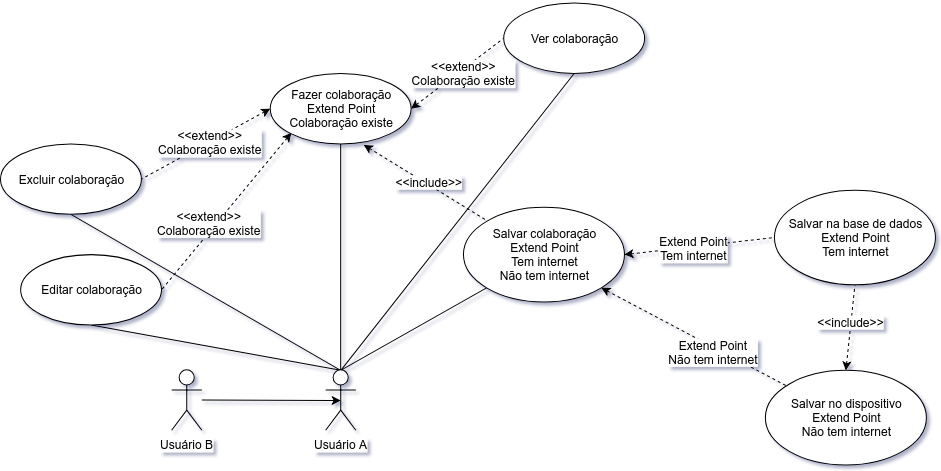
\includegraphics[width=\linewidth]{Imagens/userCase}
    	\legend{Fonte: Elaboração própria}
    	\label{fig:userCase}
    \end{figure}
    
        
    \subsection{Diagrama de classe}
O diagrama de classes na Figura \ref{fig:diagClass}, se fez necessário para entender a estrutura que o sistema possuirá, sua importância se da, uma vez que representa as classes que serão criadas na programação.
     % Diagrama de classes
    \begin{figure}[H]
    	\centering
    	\caption{Diagrama de classe.}	
    	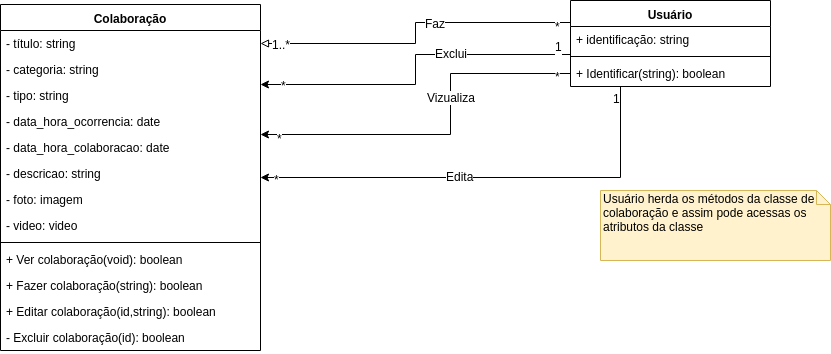
\includegraphics[width=\linewidth,]{Imagens/diagClass.png}
    	\legend{Fonte:Elaboração própria}
    	\label{fig:diagClass}
    \end{figure}
    
    
    \subsection{Diagrama de objeto}
    Este diagrama representado na Figura \ref{fig:diagObj} foi necessário para entender quais os dados que estão sendo recebidos quando o usuário realizar uma colaboração.
    % Diagrama de objeto
    \begin{figure}[H]
    	\centering
    	\caption{Diagrama de objeto.}	
    	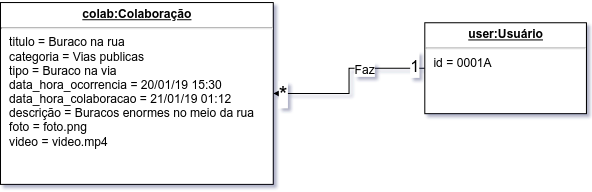
\includegraphics[width=\linewidth]{Imagens/diagObj.png}
    	\legend{Fonte:Elaboração própria}
    	\label{fig:diagObj}
    \end{figure}
    
    
    \subsection{Protótipo}
    Focou-se na criação de um protótipo interface simples e de fácil entendimento. A tela inicial \ref{fig:protInicio} é uma mensagem de boas vindas, com uma breve explicação do aplicativo. Já a \ref{fig:protMap} mostra as contribuições realizadas podendo ser visualizadas ao clicar em uma das marcas no mapa. A Figura \ref{fig:protList}, lista as colaborações realizadas, com a indicação do estado da contribuição, exclusão e edição são feitas através dos símbolos de lápis e o sinal de subtração. Por fim, a \ref{fig:protColab} é a tela de contribuição, onde o usuário preenche todas as informações e envia os dados.
    
    % Tela de inicio protótipo
    \begin{figure}[H]
    	\centering
    	\caption{Tela de inicio protótipo.}	
    	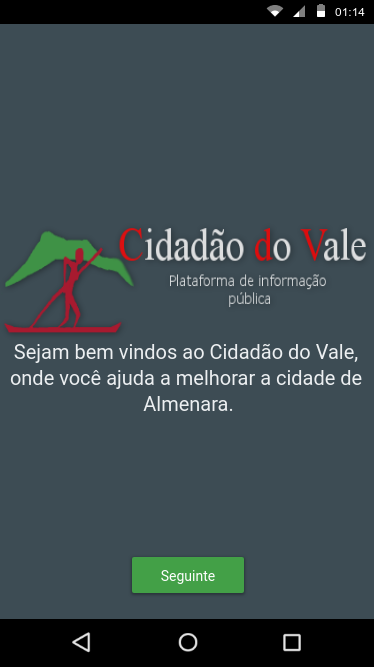
\includegraphics[width=0.6\linewidth, frame]{Imagens/protInicio.png}
    	\legend{Fonte: Elaboração própria}
    	\label{fig:protInicio}
    \end{figure}
    
    % Mapa de colaborações
    \begin{figure}[H]
    	\centering
    	\caption{Mapa de colaborações.}	
    	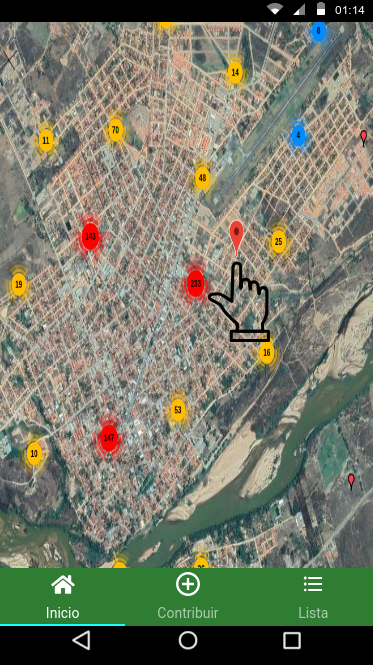
\includegraphics[width=0.6\linewidth, frame]{Imagens/protMap.png}
    	\legend{Fonte: Elaboração própria}
    	\label{fig:protMap}
    \end{figure} 
    
    % Lista de colaborações
    \begin{figure}[H]
    	\centering
    	\caption{Lista de colaborações.}	
    	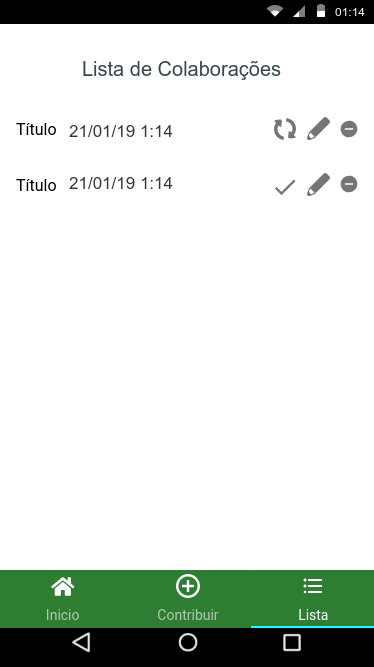
\includegraphics[width=0.6\linewidth, frame]{Imagens/protList.png}
    	\legend{Fonte: Elaboração própria}
    	\label{fig:protList}
    \end{figure}
    
    % Realizar contribuição
    \begin{figure}[H]
    	\centering
    	\caption{Realizar contribuição.}	
    	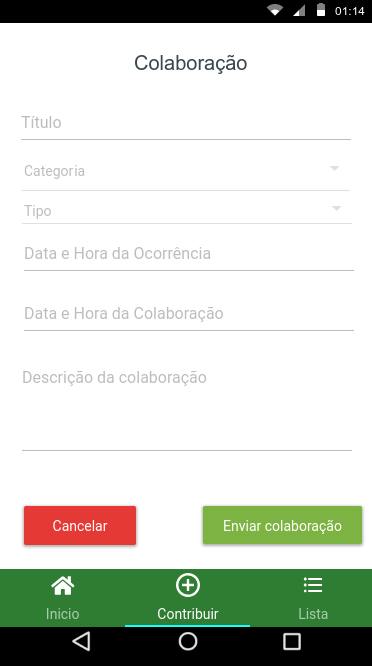
\includegraphics[width=0.6\linewidth, frame]{Imagens/protColab.png}
    	\legend{Fonte: Elaboração própria}
    	\label{fig:protColab}
    \end{figure}
    
\section{Desenvolvimento do sistema}
Esta pesquisa propõe o desenvolvimento de todas as funções da plataforma web para o mobile, inicialmente desenvolveu-se apenas a função básica de realizar contribuição que se encontra na Figura \ref{fig:app}, tornado o aplicativo apenas uma extensão do cidadão do vale que facilita as colaborações utilizando dispositivos móveis.

\begin{figure}[H]
    	\centering
    	\caption{O aplicativo versão 0.1}	
    	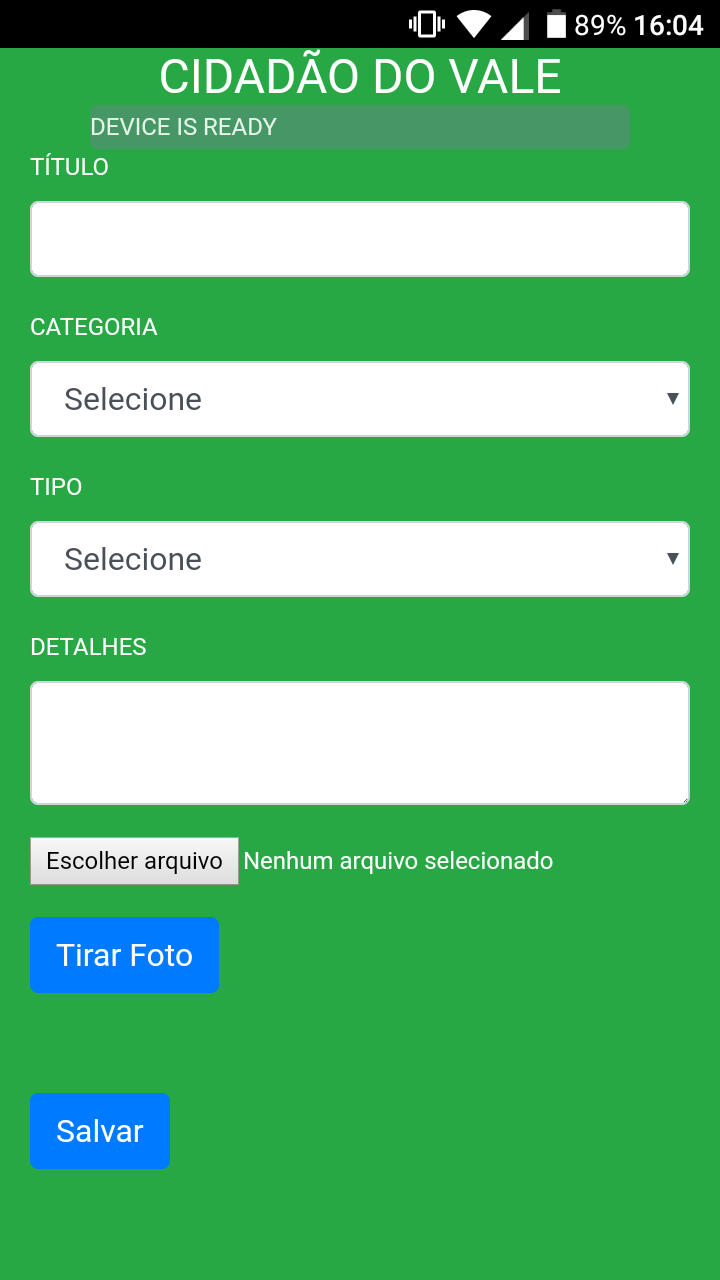
\includegraphics[width=0.6\linewidth, frame]{Imagens/app0_1.png}
    	\legend{Fonte: Elaboração própria}
    	\label{fig:app}
\end{figure}
